\documentclass[10pt]{beamer}
\usetheme{Madrid}
\usecolortheme{default}

\usepackage[utf8]{inputenc}
\usepackage[T1]{fontenc}
\usepackage{amsmath,amssymb}
\usepackage{tikz}
\usetikzlibrary{matrix,positioning,arrows.meta,shapes.geometric,calc}

\title{Projet MOGPL}
\subtitle{Navigation d'un Robot sur une Grille}
\author{Bruno Fernandes Iorio \and Gildas De Michiel}
\institute{Sorbonne Université}
\date{2025}

\begin{document}

\begin{frame}
\titlepage
\end{frame}

%======================================
\section{Problème}
%======================================

\begin{frame}{Le problème}
\begin{center}
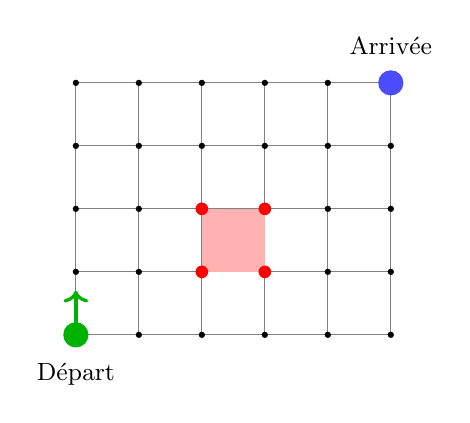
\begin{tikzpicture}[scale=0.8]
    % Grille
    \draw[step=1cm,gray,thin] (0,0) grid (5,4);
    
    % Sommets
    \foreach \x in {0,...,5} {
        \foreach \y in {0,...,4} {
            \fill[black] (\x,\y) circle (0.05);
        }
    }
    
    % Obstacle
    \fill[red!30] (2,1) rectangle (3,2);
    \fill[red] (2,1) circle (0.1);
    \fill[red] (3,1) circle (0.1);
    \fill[red] (2,2) circle (0.1);
    \fill[red] (3,2) circle (0.1);
    
    % Robot
    \fill[green!70!black] (0,0) circle (0.2);
    \draw[->,very thick,green!70!black] (0,0) -- (0,0.7);
    \node[below] at (0,-0.3) {\small Départ};
    
    % Arrivée
    \fill[blue!70] (5,4) circle (0.2);
    \node[above] at (5,4.3) {\small Arrivée};
\end{tikzpicture}
\end{center}

\vspace{0.3cm}
\textbf{Commandes :} \texttt{avancer(k)} avec $k \in \{1,2,3\}$ \quad | \quad \texttt{tourner} (G ou D)

\textbf{Objectif :} Minimiser le nombre de commandes
\end{frame}

%======================================
\section{Structure du graphe}
%======================================

\begin{frame}{Structure du graphe : 4 copies de la grille}
\begin{center}
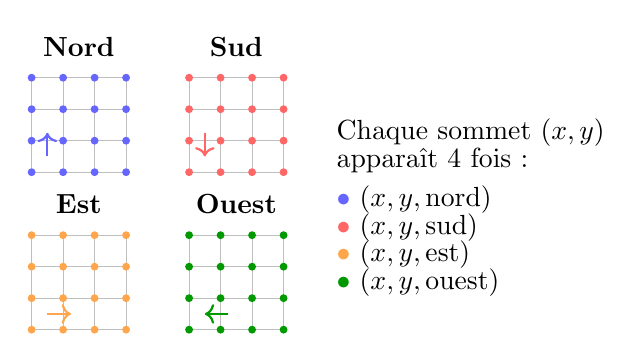
\begin{tikzpicture}[scale=0.5]
    % === NORD ===
    \begin{scope}[shift={(0,6)}]
        \draw[step=0.8cm,gray!50,thin] (0,0) grid (2.4,2.4);
        \foreach \x in {0,0.8,1.6,2.4} {
            \foreach \y in {0,0.8,1.6,2.4} {
                \fill[blue!60] (\x,\y) circle (0.1);
            }
        }
        \node[above] at (1.2,2.7) {\textbf{Nord}};
        % Flèches direction
        \draw[->,thick,blue!60] (0.4,0.4) -- (0.4,1.0);
    \end{scope}
    
    % === SUD ===
    \begin{scope}[shift={(4,6)}]
        \draw[step=0.8cm,gray!50,thin] (0,0) grid (2.4,2.4);
        \foreach \x in {0,0.8,1.6,2.4} {
            \foreach \y in {0,0.8,1.6,2.4} {
                \fill[red!60] (\x,\y) circle (0.1);
            }
        }
        \node[above] at (1.2,2.7) {\textbf{Sud}};
        \draw[->,thick,red!60] (0.4,1.0) -- (0.4,0.4);
    \end{scope}
    
    % === EST ===
    \begin{scope}[shift={(0,2)}]
        \draw[step=0.8cm,gray!50,thin] (0,0) grid (2.4,2.4);
        \foreach \x in {0,0.8,1.6,2.4} {
            \foreach \y in {0,0.8,1.6,2.4} {
                \fill[orange!70] (\x,\y) circle (0.1);
            }
        }
        \node[above] at (1.2,2.7) {\textbf{Est}};
        \draw[->,thick,orange!70] (0.4,0.4) -- (1.0,0.4);
    \end{scope}
    
    % === OUEST ===
    \begin{scope}[shift={(4,2)}]
        \draw[step=0.8cm,gray!50,thin] (0,0) grid (2.4,2.4);
        \foreach \x in {0,0.8,1.6,2.4} {
            \foreach \y in {0,0.8,1.6,2.4} {
                \fill[green!60!black] (\x,\y) circle (0.1);
            }
        }
        \node[above] at (1.2,2.7) {\textbf{Ouest}};
        \draw[->,thick,green!60!black] (1.0,0.4) -- (0.4,0.4);
    \end{scope}
    
    % Légende
    \node[right] at (7.5,7) {Chaque sommet $(x,y)$};
    \node[right] at (7.5,6.3) {apparaît 4 fois :};
    \node[right] at (7.5,5.3) {\textcolor{blue!60}{$\bullet$} $(x,y,\text{nord})$};
    \node[right] at (7.5,4.6) {\textcolor{red!60}{$\bullet$} $(x,y,\text{sud})$};
    \node[right] at (7.5,3.9) {\textcolor{orange!70}{$\bullet$} $(x,y,\text{est})$};
    \node[right] at (7.5,3.2) {\textcolor{green!60!black}{$\bullet$} $(x,y,\text{ouest})$};
\end{tikzpicture}
\end{center}

$$|V| = 4 \times (N+1) \times (M+1)$$
\end{frame}

\begin{frame}{Arcs : Avancer}
\begin{center}
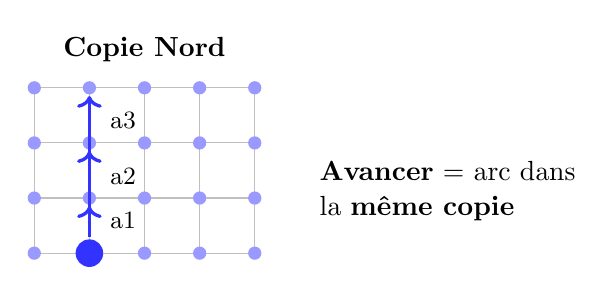
\begin{tikzpicture}[scale=0.7]
    % Grille Nord seulement
    \draw[step=1cm,gray!50,thin] (0,0) grid (4,3);
    \foreach \x in {0,...,4} {
        \foreach \y in {0,...,3} {
            \fill[blue!40] (\x,\y) circle (0.12);
        }
    }
    \node[above] at (2,3.3) {\textbf{Copie Nord}};
    
    % Robot à (1,0) orienté Nord
    \fill[blue!80] (1,0) circle (0.25);
    
    % Arcs avancer (dans la même copie)
    \draw[->,very thick,blue!80] (1,0.3) -- (1,0.85);
    \draw[->,very thick,blue!80] (1,0.3) -- (1,1.85);
    \draw[->,very thick,blue!80] (1,0.3) -- (1,2.85);
    
    % Labels
    \node[right] at (1.2,0.6) {\small a1};
    \node[right] at (1.2,1.4) {\small a2};
    \node[right] at (1.2,2.4) {\small a3};
    
    % Texte
    \node[right] at (5,1.5) {\textbf{Avancer} = arc dans};
    \node[right] at (5,0.8) {la \textbf{même copie}};
\end{tikzpicture}
\end{center}

\vspace{0.3cm}
\begin{center}
$(x, y, \text{nord}) \xrightarrow{\text{a}k} (x, y-k, \text{nord})$ \quad pour $k \in \{1,2,3\}$
\end{center}
\end{frame}

\begin{frame}{Arcs : Tourner}
\begin{center}
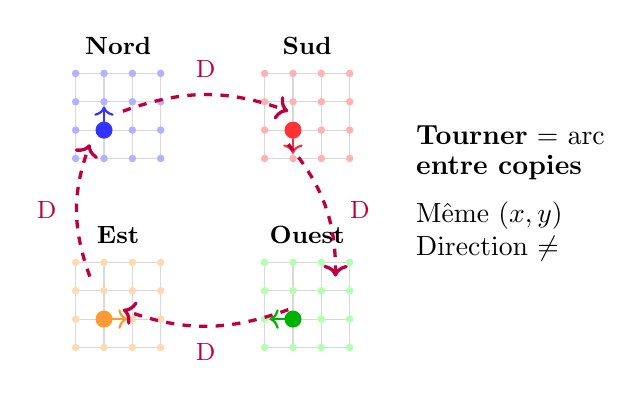
\begin{tikzpicture}[scale=0.6]
    % 4 copies avec un sommet mis en évidence
    
    % Nord
    \begin{scope}[shift={(0,4)}]
        \draw[step=0.6cm,gray!30,thin] (0,0) grid (1.8,1.8);
        \foreach \x in {0,0.6,1.2,1.8} {
            \foreach \y in {0,0.6,1.2,1.8} {
                \fill[blue!30] (\x,\y) circle (0.08);
            }
        }
        \fill[blue!80] (0.6,0.6) circle (0.18);
        \draw[->,thick,blue!80] (0.6,0.6) -- (0.6,1.1);
        \node[above] at (0.9,2) {\small\textbf{Nord}};
    \end{scope}
    
    % Sud
    \begin{scope}[shift={(4,4)}]
        \draw[step=0.6cm,gray!30,thin] (0,0) grid (1.8,1.8);
        \foreach \x in {0,0.6,1.2,1.8} {
            \foreach \y in {0,0.6,1.2,1.8} {
                \fill[red!30] (\x,\y) circle (0.08);
            }
        }
        \fill[red!80] (0.6,0.6) circle (0.18);
        \draw[->,thick,red!80] (0.6,0.6) -- (0.6,0.1);
        \node[above] at (0.9,2) {\small\textbf{Sud}};
    \end{scope}
    
    % Est
    \begin{scope}[shift={(0,0)}]
        \draw[step=0.6cm,gray!30,thin] (0,0) grid (1.8,1.8);
        \foreach \x in {0,0.6,1.2,1.8} {
            \foreach \y in {0,0.6,1.2,1.8} {
                \fill[orange!30] (\x,\y) circle (0.08);
            }
        }
        \fill[orange!80] (0.6,0.6) circle (0.18);
        \draw[->,thick,orange!80] (0.6,0.6) -- (1.1,0.6);
        \node[above] at (0.9,2) {\small\textbf{Est}};
    \end{scope}
    
    % Ouest
    \begin{scope}[shift={(4,0)}]
        \draw[step=0.6cm,gray!30,thin] (0,0) grid (1.8,1.8);
        \foreach \x in {0,0.6,1.2,1.8} {
            \foreach \y in {0,0.6,1.2,1.8} {
                \fill[green!30] (\x,\y) circle (0.08);
            }
        }
        \fill[green!70!black] (0.6,0.6) circle (0.18);
        \draw[->,thick,green!70!black] (0.6,0.6) -- (0.1,0.6);
        \node[above] at (0.9,2) {\small\textbf{Ouest}};
    \end{scope}
    
    % Flèches de rotation entre les copies
    \draw[->,very thick,purple,dashed] (1.0,5.0) to[bend left=20] (4.5,5.0);
    \node[above,purple] at (2.75,5.5) {\small D};
    
    \draw[->,very thick,purple,dashed] (4.5,4.3) to[bend left=20] (5.5,1.5);
    \node[right,purple] at (5.6,2.9) {\small D};
    
    \draw[->,very thick,purple,dashed] (4.5,0.8) to[bend left=20] (1.0,0.8);
    \node[below,purple] at (2.75,0.3) {\small D};
    
    \draw[->,very thick,purple,dashed] (0.3,1.5) to[bend left=20] (0.3,4.3);
    \node[left,purple] at (-0.2,2.9) {\small D};
    
    % Légende
    \node[right] at (7,4.5) {\textbf{Tourner} = arc};
    \node[right] at (7,3.8) {\textbf{entre copies}};
    \node[right] at (7,2.8) {Même $(x,y)$};
    \node[right] at (7,2.1) {Direction $\neq$};
\end{tikzpicture}
\end{center}
\end{frame}

\begin{frame}{Rotation : vue détaillée}
\begin{center}
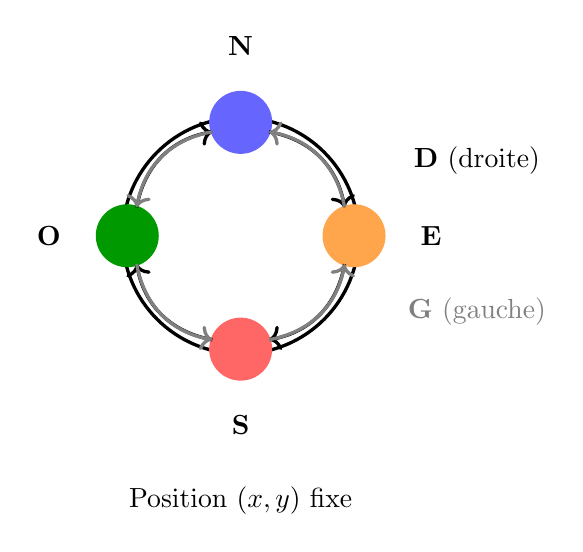
\begin{tikzpicture}[scale=1.2]
    % Cercle central
    \node[circle,draw,very thick,minimum size=3cm] (center) at (0,0) {};
    
    % 4 états
    \node[circle,fill=blue!60,minimum size=0.8cm] (N) at (0,1.2) {};
    \node[above] at (0,1.8) {\textbf{N}};
    \draw[->,thick,blue!60] (0,1.0) -- (0,1.5);
    
    \node[circle,fill=red!60,minimum size=0.8cm] (S) at (0,-1.2) {};
    \node[below] at (0,-1.8) {\textbf{S}};
    \draw[->,thick,red!60] (0,-1.0) -- (0,-1.5);
    
    \node[circle,fill=orange!70,minimum size=0.8cm] (E) at (1.2,0) {};
    \node[right] at (1.8,0) {\textbf{E}};
    \draw[->,thick,orange!70] (1.0,0) -- (1.5,0);
    
    \node[circle,fill=green!60!black,minimum size=0.8cm] (O) at (-1.2,0) {};
    \node[left] at (-1.8,0) {\textbf{O}};
    \draw[->,thick,green!60!black] (-1.0,0) -- (-1.5,0);
    
    % Arcs D (sens horaire, extérieur)
    \draw[->,very thick,black] (0.3,1.1) to[bend left=35] (1.1,0.3);
    \draw[->,very thick,black] (1.1,-0.3) to[bend left=35] (0.3,-1.1);
    \draw[->,very thick,black] (-0.3,-1.1) to[bend left=35] (-1.1,-0.3);
    \draw[->,very thick,black] (-1.1,0.3) to[bend left=35] (-0.3,1.1);
    
    \node at (2.5,0.8) {\textbf{D} (droite)};
    
    % Arcs G (sens anti-horaire, intérieur)
    \draw[->,very thick,gray] (-0.3,1.1) to[bend right=35] (-1.1,0.3);
    \draw[->,very thick,gray] (-1.1,-0.3) to[bend right=35] (-0.3,-1.1);
    \draw[->,very thick,gray] (0.3,-1.1) to[bend right=35] (1.1,-0.3);
    \draw[->,very thick,gray] (1.1,0.3) to[bend right=35] (0.3,1.1);
    
    \node at (2.5,-0.8) {\textcolor{gray}{\textbf{G} (gauche)}};
    
    % Position
    \node at (0,-2.8) {Position $(x,y)$ fixe};
\end{tikzpicture}
\end{center}
\end{frame}

%======================================
\section{Structures de données}
%======================================

\begin{frame}{Structures de données}
\textbf{Classe \texttt{Node} :}
\begin{itemize}
    \item \texttt{(x, y, orientation)}
    \item \texttt{next[ ]} : liste des successeurs
\end{itemize}

\vspace{0.5cm}
\textbf{Classe \texttt{Graph} :}
\begin{itemize}
    \item \texttt{Nodes} : dictionnaire $\{(x,y,dir) \to \text{Node}\}$
    \item \texttt{blockedList} : sommets bloqués
\end{itemize}

\vspace{0.5cm}
\textbf{Obstacle :} une cellule $(i,j)$ bloque 4 sommets

\begin{center}
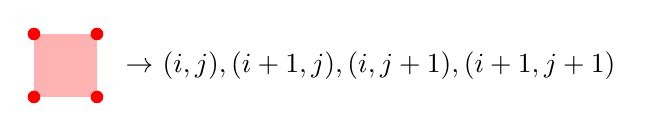
\begin{tikzpicture}[scale=0.8]
    \fill[red!30] (0,0) rectangle (1,1);
    \fill[red] (0,0) circle (0.1);
    \fill[red] (1,0) circle (0.1);
    \fill[red] (0,1) circle (0.1);
    \fill[red] (1,1) circle (0.1);
    \node[right] at (1.3,0.5) {$\to$ $(i,j), (i+1,j), (i,j+1), (i+1,j+1)$};
\end{tikzpicture}
\end{center}
\end{frame}

%======================================
\section{Algorithme BFS}
%======================================

\begin{frame}{Algorithme BFS}
\begin{center}
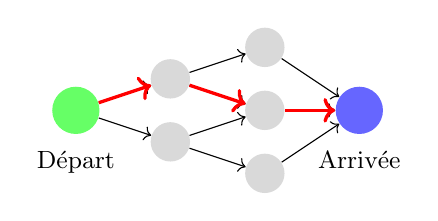
\begin{tikzpicture}[scale=0.8]
    % Graphe simplifié
    \node[circle,fill=green!60,minimum size=0.6cm] (start) at (0,0) {};
    \node[below] at (0,-0.5) {\small Départ};
    
    \node[circle,fill=gray!30,minimum size=0.5cm] (a) at (1.5,0.5) {};
    \node[circle,fill=gray!30,minimum size=0.5cm] (b) at (1.5,-0.5) {};
    \node[circle,fill=gray!30,minimum size=0.5cm] (c) at (3,1) {};
    \node[circle,fill=gray!30,minimum size=0.5cm] (d) at (3,0) {};
    \node[circle,fill=gray!30,minimum size=0.5cm] (e) at (3,-1) {};
    \node[circle,fill=blue!60,minimum size=0.6cm] (end) at (4.5,0) {};
    \node[below] at (4.5,-0.5) {\small Arrivée};
    
    \draw[->] (start) -- (a);
    \draw[->] (start) -- (b);
    \draw[->] (a) -- (c);
    \draw[->] (a) -- (d);
    \draw[->] (b) -- (d);
    \draw[->] (b) -- (e);
    \draw[->] (c) -- (end);
    \draw[->] (d) -- (end);
    \draw[->] (e) -- (end);
    
    % Chemin optimal
    \draw[->,very thick,red] (start) -- (a);
    \draw[->,very thick,red] (a) -- (d);
    \draw[->,very thick,red] (d) -- (end);
\end{tikzpicture}
\end{center}

\vspace{0.3cm}
\begin{itemize}
    \item Graphe \textbf{non pondéré} $\Rightarrow$ BFS = optimal
    \item Parcours en largeur depuis $(x_0, y_0, dir_0)$
\end{itemize}

\vspace{0.3cm}
$$\text{Complexité : } O(|V| + |E|) = O(N \times M)$$
\end{frame}

\begin{frame}{Résultats expérimentaux}
\begin{columns}
\begin{column}{0.5\textwidth}
\textbf{(c) Taille de la grille $\times$ temps de resolution (bfs):}
\begin{center}
\begin{tabular}{|c|c|}
\hline
Taille & Temps (s) \\
\hline
$10 \times 10$ & 0.000897 \\
$20 \times 20$ & 0.010343 \\
$30 \times 30$ & 0.050940 \\
$40 \times 40$ & 0.222723 \\
$50 \times 50$ & 0.530197 \\
\hline
\end{tabular}
\end{center}
\end{column}
\begin{column}{0.5\textwidth}
\textbf{(d) Nombre d'obstacles $\times$ temps de génération du graphe:}
\begin{center}
\begin{tabular}{|c|c|}
\hline
Obstacles & Temps (s) \\
\hline
10 & 0.012374 \\
20 & 0.007275 \\
30 & 0.008942 \\
40 & 0.006518 \\
50 & 0.002126 \\
\hline
\end{tabular}
\end{center}

\end{column}
\end{columns}
\end{frame}

%======================================
\section{Génération d'obstacles (PLNE)}
%======================================

\begin{frame}{Génération d'obstacles par PLNE}
\textbf{Variables :} $x_{i,j} \in \{0,1\}$, \quad $w_{i,j} \in [0,1000]$ (aléatoire)

\vspace{0.3cm}
$$\min \sum_{i,j} x_{i,j} \cdot w_{i,j}$$

\vspace{0.3cm}
\textbf{Contraintes :}
\begin{itemize}
    \item $\sum_{i,j} x_{i,j} = P$ \quad (exactement $P$ obstacles)
    \item $\sum_j x_{i,j} \leq 2P/M$ \quad (par ligne)
    \item $\sum_i x_{i,j} \leq 2P/N$ \quad (par colonne)
    \item $x_{i,j} + x_{i,j+2} - x_{i,j+1} \leq 1$ \quad (pas de 1-0-1 horizontal)
    \item $x_{i,j} + x_{i+2,j} - x_{i+1,j} \leq 1$ \quad (pas de 1-0-1 vertical)
\end{itemize}

\vspace{0.3cm}
\textbf{Complexité :} PLNE $\Rightarrow$ NP-difficile, mais Gurobi résout rapidement
\end{frame}

%======================================
\section{Conclusion}
%======================================

\begin{frame}{Conclusion}
\begin{center}
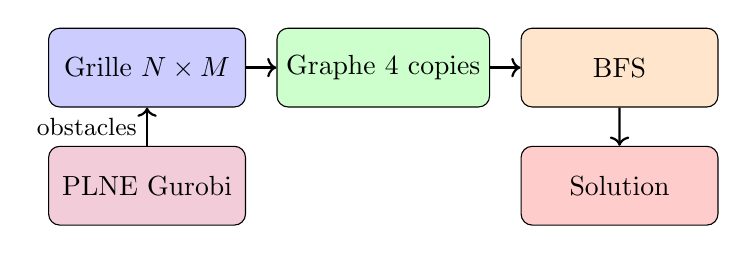
\begin{tikzpicture}[scale=0.6]
    % Schéma récapitulatif
    \node[draw,rounded corners,fill=blue!20,minimum width=2.5cm,minimum height=1cm] (grille) at (0,0) {Grille $N \times M$};
    \node[draw,rounded corners,fill=green!20,minimum width=2.5cm,minimum height=1cm] (graphe) at (5,0) {Graphe 4 copies};
    \node[draw,rounded corners,fill=orange!20,minimum width=2.5cm,minimum height=1cm] (bfs) at (10,0) {BFS};
    \node[draw,rounded corners,fill=red!20,minimum width=2.5cm,minimum height=1cm] (sol) at (10,-2.5) {Solution};
    \node[draw,rounded corners,fill=purple!20,minimum width=2.5cm,minimum height=1cm] (plne) at (0,-2.5) {PLNE Gurobi};
    
    \draw[->,thick] (grille) -- (graphe);
    \draw[->,thick] (graphe) -- (bfs);
    \draw[->,thick] (bfs) -- (sol);
    \draw[->,thick] (plne) -- node[left]{\small obstacles} (grille);
\end{tikzpicture}
\end{center}

\vspace{0.5cm}
\begin{itemize}
    \item \textbf{Graphe :} 4 copies $\times$ $(N+1)(M+1)$ sommets
    \item \textbf{BFS :} $O(NM)$
    \item \textbf{Obstacles :} PLNE avec distribution équilibrée
\end{itemize}

\vspace{0.3cm}
\begin{center}
\textbf{Merci !}
\end{center}
\end{frame}

\end{document}
